
\chapter{Description of our prototype for spatio-angular illumination}
\label{sec:dev1}
\begin{summary}
  In the preceding chapter I showed the underlying concept of our
  spatio-angular microscope. Here I discuss additional details that
  are important for the practical implementation.

  I explain the beam path, electronic synchronization of the displays
  with other components and an algorithm to transform the coordinate
  system of the camera pixels into the coordinate system of the focal
  plane SLM.
  
  The pupil plane SLM was specifically developed for our project by    
  our partner Fraunhofer IPMS (Dresden, DE). 
  % FIXME more on mma?
\end{summary}
\section{Description of the optical components}
In chapter \ref{sec:concept} I have shown the beam path for
transmissive displays (in \figref{fig:memi-simple}). Such SLM have a
very low transmission in practice. Therefore we use reflective
displays in our prototype.

In \figref{fig:memi-real} I adjusted the beam path accordingly. This
schematic also depicts the optics we use to adapt light from the laser
to fill the etendue of our system. The light source enters the system
from the bottom left. The optic components are color corrected and
have anti-reflex coating for wavelengths in the range from
\unit[400]{nm} to \unit[700]{nm}.

The system successively illuminates the pupil plane SLM --- a greyscale
micromirror array developed by our project partner Fraunhofer IPMS
Dresden --- and the focal plane SLM, a commercial binary liquid crystal
on silicon display.
 
\begin{figure}[!htbp]
  \centering
  \svginput{2}{memi-real}
  \caption{Schematic of the light path through our microscope. Laser
    light enters from the lower left, is scrambled and homogenized to
    illuminate the pupil plane SLM in $\textrm{P}''$ and the focal
    plane SLM in $F'$. $F$ is the field plane in the sample and its
    primed versions are conjugated planes. $P$ is the pupil of the
    objective. Field mask $B_0$ and Fourier stop $B_1$ are adjustable
    circular apertures. PBS is a polarizing beam splitter. DBS is a
    dichroic beam splitter.  The red boxes deliminate subsystems of
    the illumination system: {\color{Orchid}\bf A$_1$ and A$_2$:}
    light scrambling and homogenization, {\color{Orchid}\bf B:}
    Fourier-optical filter to provide intensity modulating pupil plane
    SLM. {\color{Orchid}\bf C:} Polarization based intensity modulator
    as focal plane SLM. {\color{Orchid}\bf D:} Wide-field fluorescence
    microscope with detection path.}
  \label{fig:memi-real}
\end{figure}

\subsection{Ensuring homogeneous illumination}
A quantitative evaluation of our experiments (section
\ref{sec:results}) with different illumination patterns is simplified
when both pupil plane SLM and focal plane SLM are uniformly
illuminated.  Below we discuss an optical setup that attains
homogeneity of the illumination of both displays.

We use either a laser\footnote{Lasever LSR473H, diode-pumped solid
  state laser, output power 600mW, $\lambda=\unit[473]{nm}$} or a
light emitting diode (LED) as the light source in our experiments. The
LED\footnote{Huey Jann HPB8-48KBD, wavelength $\unit[(463\pm1)]{nm}$,
  brightness \unit[35]{lm}, view angle
  $120{}^\circ$ %, FIXME TODO: Flaeche messen
} we use has a large active area.  Due to etendue mismatch a
relatively large amount of light will never reach the sample. However,
it is easy to achieve a homogeneous illumination with an
LED. Moreover, the LED can be quickly switched on and off
electronically. Nevertheless, it would be better to use an LED with a
smaller active area but those are hard to find.
% source code: https://github.com/plops/ledtlc/blob/master/ledtlc.ino

 % \footnote{The DPSS Laser doesn't allow fast
 %  direct electronic switching at full power. We have to use an
 %  acousto-optic modulator connected with the additional expense of its
 %  optical alignment (FIXME siehe spaetere ref section).}.

Unlike an LED, a laser delivers light of considerably higher spectral
radiance ($\unit[]{W/(sr\, m^2 m)}$). Thus it is in principle possible
to use the laser as a highly efficient light source for our
system. Unfortunately, the high spectral and spatial coherence of a
laser often leads to high-contrast fluctuations of the irradiance and
we have to compensate for this by time averaging.

When using the laser, we send its collimated Gaussian beam into a
bundle\footnote{Fiber bundle with circular cross-section (Loptek,
  Berlin, DE), \unit[1.1]{mm} diameter and \unit[2]{m} length. The
  beam broadening is $3{}^\circ$ and increases, when the bundle is
  bent \citep{Ipp2009}.}  of randomly distributed fibers. This
randomizes the light distribution at the bundle output and also
broadens the illumination angles.

A relay system (A$_1$ in \figref{fig:memi-real}) images the circular
output of the fiber bundle onto the entrance of a light pipe. This
relay system contains a rotating microlens array\footnote{Array of
  cross-oriented cylindrical lenses on both sides with a pitch of
  \unit[0.5]{mm} resulting in an effective focal length of
  \unit[6.9]{mm} (LIMO, Dortmund, DE).}. It is driven by a motor with
the axis of rotation displaced from the optical axis. Integrating
sufficiently long over the time-variations in the intensity pattern
allows to reduce speckle.

Both the fiber bundle and microlens array increase the etendue of the
laser illumination to the optimum value, which is given by one of our
SLM as discussed on page \pageref{sec:etendue-mma}.

The integration tunnel shown in \figref{fig:integrator-rod} is hollow
and has a quadratic cross-section. The mixing effect of the tunnel can
be understood by considering the irradiance in the plane of the tunnel
output as it would occur without tunnel.  Drawing the outline of the
square cross-section into this irradiance map selects the light that
reaches this plane directly without any reflection.  Surrounding this
outline with four identical copies that touch its edges selects the
light that will reach the output plane after one reflection. The
irradiance maps from neighbouring squares are mirrored and added to
the direct illumination. Depending on the numerical aperture of the
input light, more reflections may occur --- resulting in the addition
of irradiance from next-nearest-neighbours.

This integration tunnel improves the uniformity of the light
distribution in the output plane without altering the numerical
aperture of the light.  The more subregions are superimposed, the
better will be the uniformity of the illumination.  Assuming $N$
subregions were overlaid and their contributions were statistically
independent, then according to the central limit theorem the standard
deviation of the irradiance is proportional to $1/\sqrt{N}$
\citep{Koshel2012}. {\color{red} FIXME ondrej says this comes directly
  from poisson distribution but i don't think so}

We also align the source distribution to be rotationally symmetric
about the optical axis and obtain an even more uniform output because
positive and negative slopes from different subregions compensate in
the superposition (also \cite{Koshel2012}).

The dimensionis of the integration tunnel in our sytem is
$\unit[2.5]{mm}\times\unit[2.5]{mm}\times\unit[250]{mm}$ and ensures
enough reflections for homogeneous illumination. A relay system
magnifies the tunnel output to $\unit[4]{mm}\times\unit[4]{mm}$ in the
plane $\textrm{F}'''$.

\jpginput{8cm}{integrator-rod}{Hollow mirror-integrator tunnel with a
  quadratic cross section of \unit[2.5]{mm} side length and
  \unit[250]{mm} length.}


During the planning phase we also considered a homogenization design
based on a fly's eye condensor (two consecutive microlens
arrays). According to simulations performed by In-Vision, this,
however, would have been more difficult to adjust than the tunnel. In
particular the system would have been more dependent on illumination
wavelength compared to the tunnel.

In summary the following points are important in order to achieve
homogeneous illumination of focal and pupil plane with the tunnel:
%\renewcommand{\labelitemi}{$\star$}
\begin{itemize}
\item The image of the end of the bundle should properly cover the
  tunnel entrance. Especially the corners of the tunnel should not be
  darker than the center. Inhomogeneous illumination at the tunnel
  entrance leads to inhomogeneous illumination of the pupil plane SLM.
\item The end of the fibre bundle must be adjusted in four axes
  (centering and angle).
\item The focal length of the microlenses should be chosen shorter
  than predicted by pure etendue calculation in order to compensate
  microchipping (FIXME better word) on the edges of the cemented glass
  mirrors.
\end{itemize}

\subsection{Fourier optical filter for contrast generation on pupil
  plane SLM}
\label{ref:mma}
The micromirror array, which we use as a pupil plane SLM consists of
torsion mirrors that modulate the phase of the light (see
\figref{fig:mma} for images of the device). In order to modulate the
intensity we use the Fourier optical filter denoted as
'schlierenoptics' in \figref{fig:memi-real}~B.

The device itself is documented in more detail the following
references: design of the actuators \citep{Schmidt2010}, grey value
images and contrast measurement \citep{Berndt2010} and per-pixel
calibration of the deflection angle using a white light interferometer
\citep{Berndt2011,Berndt2007}.

\jpginput{14cm}{mma}{{\bf left:} Scanning electron microscope image of
  the micro-mirror array (MMA).  The pixel pitch of the device is
  \unit[0.016]{mm}. The hinges for the tilt movement and the
  electrodes are clearly visible. {\bf middle:} Optical reflective
  microscope image of the MMA. {\bf right:} Rendering of how a 8x8
  checker board pattern would be displayed on the device. The
  deflection angles are exaggerated.  Electron and optical micrograph
  by Fraunhofer IPMS Dresden (Germany)}

The lens L1 has two purposes: First, it images the field mask B0 into % FIXME is it capital F after colon?
the Fourier stop B1. Second, the plane $\textrm{P}''$ with the phase
SLM is imaged to infinity.

With undeflected micromirrors, the SLM has no signifcant effect and
works like a plane mirror. Both planes $\textrm{F}''$ and
$\textrm{P}'$ are then homogeneously illuminated.

If the left half of the micromirrors are tilted, then they direct the
light along the dashed line in \figref{fig:memi-real}. This light is
absorbed by the field stop B1 and therefore missing in $\textrm{P}'$,
i.e.\ the right side in $\textrm{P}'$ is dark. The total radiant flux
($\unit[]{W}$) through the beam stop in $\textrm{F}''$ decreases while
the transmitted irradiance ($\unit[]{W/m^2}$) remains homogeneous.  In
the real system, the lens L1 consists of four glass elements.

FIXME translate: Beschreibe den Effekt des MMA Gratings auf eine
monochromatische Ebene Welle.  Um das Fouriermuster zu beschreiben
betrachte ich zunaechst einzelnes Pixel mit Breite $w=\unit[16]{\mu
  m}$. Dieses laesst sich zunaechst in einer Dimension durch den
folgenden Ausdruck beschreiben:
\begin{align}
  T_p(x)=\delta(x-x_p)\otimes\left(\rect(x/w)\cdot e^{i k_p x}\right)\quad\textrm{with}\ \rect(x):=\begin{cases} 1 & |x|<1/2 \\ 0 & \textrm{else} \end{cases}
\end{align}
Die Faltung mit der $\delta-$Funktion schiebt das Pixel an die Stelle
$x_p$ und $k_p$ beschreibt den Kippwinkel des Spiegels. Mit der
Fouiertransformation
\begin{align}
  \frac{1}{w}\int_{-w/2}^{w/2} e^{ikx} \textrm{d}x =
  \frac{\sin(kw/2)}{kw/2} =: \sinc(kw/2)
\end{align}
ergibt sich das Fraunhofer Beugungsbild eines einzelnen Pixels zu:
\begin{align}
  \widetilde T_p(k_x) = e^{ik_x x_p} \left(w \sinc(kw/2)\otimes\delta(k_x-k_p)\right)
\end{align}
D.h. das sinc-foermige Beugungsbild des Pixels verschiebt sich im
k-Raum, je nach deflection des Spiegels.

Angenommen die $N$ Pixel sind entlang einer Zeile mit einem Pitch
verteilt, der identisch ihrer Breite ist, also $x_p=w\cdot p$ mit
$p\in \big[-\lfloor N/2\rfloor,\lfloor N/2\rfloor+1\big]$ wobei
$\lfloor N/2\rfloor$ die groesste ganze Zahl beschreibt, die kleiner
N/2 ist.  Der Einfachheit halber vernachlaessige ich die Spalte
zwischen den Spiegeln (sie Elektronenmikroskopbild).  Das
Fourierspektrum $\widetilde T_\textrm{line}$ dieser Zeile:
\begin{align}
  \widetilde T_\textrm{line}(k_x) & = \sum_{p=-\lfloor N/2\rfloor}^{\lfloor N/2\rfloor+1} T_p(k_x) 
  = \sum_{p=-\lfloor N/2\rfloor}^{\lfloor N/2\rfloor+1} e^{ik_x w p} \left(w
    \sinc(k_x w/2)\otimes\delta(k_x-k_p)\right)
\end{align}
Dieser Ausdruck ist die Fouriertransformation eines Liniengitters mit
dem Pixelpitch als Periode, moduliert mit den einzelnen sinc
Funktionen. Im ersten Diagramm ist nur der Absolutsquare der Summe
ueber den Phasenfaktor $\sum_p exp(ik_x w p)$ fuer $N=2$ und $N=20$
dargestellt.  Der von uns verwendete Spiegel hat $N=256$, d.h. die
Summe liefert einen Zug sehr feiner Beugungsordnungen.

Im naechsten Bild ist der volle Ausdruck $\widetilde
T_\textrm{line}(k_x)$ dargestellt (wieder fuer $N=20$).  Dabei habe
ich die Spiegeldeflectionen mittels $k_p$ variiert.  Der Fall $k_p$
entspricht der roten Linie. In diesem Fall sind alle Spiegel
unausgelenkt und alles Licht bleibt in der nullten Ordnung. Ein
besonders interessanter Fall tritt fuer $k_p=\pi$ auf. Dies entspricht
der Blazekondition und der Abstand zweier benachbarter Spiegelkanten
betraegt $\lambda/2$. Bei der Reflexion wird alles Licht (der
entsprechenden Wellenlaenge) in die erste Ordnung reflektiert.

Im naechsten Diagramm ist die Intensitaet in der nullten Ordnung fuer
variierende Spiegelkippung dargstellt. Dieses
\begin{align}
  |\widetilde T_\textrm{line}(0)|^2 = \sinc(k_p)^2
\end{align}
% block([N:20,dx:3,k:0],plot2d(cabs(sum(exp(%i*k*p*dx)*sinc(k*dx/2+kp),p,-N/2,N/2+1))^2,[kp,0,%pi*2]));

Bei der Fourierfilterung soll 

\begin{figure}[!hbt]
  \centering
  \includegraphics{diffraction_lines}
  \includegraphics{diffraction_rects}
  \includegraphics{diffraction_kp}
  \caption{ vcasdfa}
  \label{fig:maxima-diffraction}
\end{figure}


\begin{figure}[!hbt]
  \centering
  \svginput{.6}{mma-fft}
  \caption{{\bf left:} Measurement of the deflection of micro-mirrors
    using a white-light interferometer (provided by Fraunhofer IPMS
    Dresden (Germany)). {\bf right:} Simulation of the Fraunhofer
    diffraction pattern of the micro-mirror array for coherent,
    monochromatic light (kindly provided by Joel Seligson). The
    circles with radius $d_\textrm{max}$ indicate the maximum size of
    the field mask B0 where the diffraction orders do not
    overlap. This limits the etendue of our illumination system.}
  \label{fig:mma-fft}
\end{figure}


The phase distribution $\Phi(\x)$ in MMA plane corresponds to the       \cma{Fourier diffraction pattern}
profile in \figref{fig:mma-fft}~left:
\begin{align}
\label{eq:mma-complex}
 \Phi(\x) =  \sum_\p \left[\underbrace{\left(\exp(i \k(p_x,p_y) \x)\cdot \rect(x,y)\right)}_{\Phi_\p}\otimes
  \delta(x-p_x\Delta x, y-p_y\Delta y)\right]
\end{align}
where $\x=(x,y)$ is a position in the MMA plane, the rectangular
function $\rect$ delimits an individual micro-mirror with its
deflection encoded in $\k=(k_x,k_y)^T$. The index vector
$\p=(p_x,p_y)^T$ indicates the mirror position.

The diffraction pattern of an individual mirror is a $\sinc-$function
which is shifted according to the mirror deflection and a phase
gradient which depends on the mirror position $\p$: {\color{red} FIXME  expand explanation}
\begin{align}
 \widetilde\Phi_\p(\k)=\mathcal{F}(\Phi_\p(\x)) = \sinc\left(k_x-k(p_x,p_y)\right) \cdot\exp\left(i\k(p_x\Delta x,p_y \Delta y)\right)
\end{align}
Adjacent rows of mirrors tilt in opposite directions ($\pm x$).
Therefore, we can specify the term $\Phi_\p(\x)$ in equation
\ref{eq:mma-complex}:
FIXME specify k0
\begin{align} 
  \Phi_\p^{(1)}(x)&=e^{+i\k_0\x}\rect(x)\otimes\sum_p\delta(x-p\Delta x) \\
  \Phi_\p^{(2)}(x)&=e^{-i\k_0\x}\rect(x)\otimes\sum_p\delta(x-p\Delta x) 
\end{align}
An analytical description of the MMA surface is:
\begin{align}
  \Phi(\r)&=\Phi_\p^{(1)}(x) \left(\rect(y')\otimes\sum\textrm{(every second row)}\right)(y) \nonumber \\
  &\qquad+\Phi_\p^{(2)}(x) \left(\rect(y')\otimes\sum\textrm{(every second row, shifted by one)}\right)
\end{align}
\figref{fig:mma-fft}~right shows a numerically calculated diffraction
pattern of this structure for a monochromatic plane wave. Suppose the
Fourier stop B1 blocks light outside of the circle with the solid
line. Then the transmitted zero-order irradiance is proportional to
the $\sinc^2$ of the deflection angle.  This approximately applies
even if not all mirrors of the array are deflected. Therefore, we can
modulate the irradiance in the plane $P'$ using this optical system
albeit the transfer function is non-linear.

An accurate prediction of the irradiance in $P'$ is more difficult to
describe when the field mask B0 is opened and the extended source
produces illumination that is spatially partially coherent
\citep{Mehta2010a}. However, the contrast can only achieve good
results \cma{maximal etendue} if the first diffraction orders (dashed
circles in \figref{fig:mma-fft}~right) can not pass the Fourier stop
B1. This limits the size of the field mask B0 to the diameter
$d_\textrm{max}$, assuming that no high frequency pattern is displayed
on the MMA.

The smallest distance between the orders in
\figref{fig:mma-fft}~right \label{sec:etendue-mma} corresponds to a
size $\Lambda$ of two mirror pitches: $\Lambda=\unit[32]{\mu
  m}$. Therefore, the diffraction angle $\theta$ is:
\begin{align}
  \sin\theta&=\lambda/\Lambda
\end{align}
Therefore, we can express the maximum radius:
\begin{align}
  d_\textrm{max} &= f_\textrm{L1} \tan\theta \approx \frac{f\lambda}{\Lambda}
\end{align}
Here, $f_\textrm{L1}$ is the focal length of lens L1. With the
F-number $\#=f_\textrm{L1}/(2d_\textrm{max})$ we can find the maximum
etendue of the Fourier optical system:
% f/(2*f l/L) = L/(2*l)
\begin{align}
\mathcal{E} = \frac{\pi A}{4 \#^2} = \frac{\pi A\lambda^2}{\Lambda^2},  
\end{align}
with the area $A=(\unit[4]{mm})^2$ of the micro-mirror array.


% (%i1) 16*%pi*.4^2/32^2,numer;
% (%o1)                         .007853981633974483
% (%i2) 16*%pi*.7^2/32^2,numer;
% (%o2)                         .02405281875404685

For our system the maximal etendue is between $\unit[0.0079]{mm^2/sr}$
and $\unit[0.024]{mm^2/sr}$, depending on the wavelength. This is much
smaller than the etendue of a typical microscope objective
($\unit[0.27]{mm^2/sr}$, see section \ref{sec:etendue}) and
corresponds to a field diameter $D_\textrm{field}$ in the specimen
between $\unit[70]{\mu m}$ for a wavelength $\lambda$ of
\unit[400]{nm} and $\unit[125]{\mu m}$ for \unit[700]{nm}, with
\begin{align}
  D_\textrm{field}=\frac{2}{\textrm{NA}}\sqrt{\frac{\mathcal{E}}{\pi}},
\end{align}
where $\textrm{NA}$ is the numerical aperture.

% NA:1.4; eps:0.0079; sqrt(eps/(NA^2*%pi/4)),numer;
% NA:1.4; eps:0.024; sqrt(eps/(NA^2*%pi/4)),numer;


%\jpginput{14cm}{mma-calib}{bal}


\subsection{Relay optics between pupil plane and focal plane SLM}
The lenses L2 and L3 form a double-telecentric relay system with
magnification 2 and image $\textrm{F}''$ onto the focal plane SLM in
$\textrm{F}'$. At the same time these lenses make sure that the pupil
plane SLM is imaged to infinity.
 
The relay system ensures that the pixels of the focal plane SLM (see
\figref{fig:memi-real}) are at the resolution limit, while the pupil
plane SLM fills the pupil.  In addition, the relay system enables a
simpler mechanical realization and good contrast. It would be
difficult to accommodate the focal plane SLM and polarization beam
splitter in $\textrm{F}''$. Attaching an adjustable aperture would
probably not be feasible at all.


\subsection{ Contrast generation on focal plane SLM using
  polarization}
The SLM we use to control the focal plane illumination is a \cma{Why
  fLCoS and not DMD?}  ferroelectric liquid crystal on silicon device
(fLCoS, ForthDD WXGA R3, UK). If a pixel is off the returning light
retains its polarization. If a pixel is on, the polarization of the
light is rotated by 90 degrees \citep{Martinez-Garcia2009}.  From
this, a polarization beam splitter generates a binary intensity
contrast (see \figref{fig:memi-real}~C).

We have not used a digital micro-mirror device (DMD), because those
mirrors have sharp edges and loose significant amounts of light into
higher orders that can not contribute to the image in the
specimen. The pixels borders of a fLCoS device are defined by electric
fields and are therefore more blurred. In this sense, an fLCoS based
device should be more efficient than a DMD.

We use a wire-grid polarization beam splitter (Moxtek PBF02C,     \cma{polarizing beam splitter}
Orem, UT, US) because they ensure a high enough optical quality, good
contrast and the plate causess less back reflections than a beam
splitter cube.


%- ignacio moreno 2009 operational modes of a ferroelectric lcos
%(FIXME)

The s-polarized component of the incoming light is reflected towards
the SLM. Active pixels of the SLM rotate the polarization of light by
90 degrees. The light then passes through the beam splitter as
p-polarization in the direction of the microscope. There is a
supplementary cleanup analyzer in the beam path.

It would also be conceivable to arrange SLM and beam splitter
differently, so that the light coming from the SLM is \emph{reflected}
towards the microscope. In this case, however, unwanted bending of the
beam splitter's surface would deteriorate the image quality of the
focal plane SLM. Therefore, we use the beam splitter in transmission.


% The beam splitter plate makes the overall optics slightly asymmetric
% and thus induces astigmatism and lateral color \citep{Ipp2009a}. The
% plate is thin enough (thickness \unit[0.7]{mm}), so that the design
% remains diffraction limited.

 	
\jpginput{14cm}{setup-photo-blueprint}{The wide field epi-fluorescence
  microscope with attached illumination head. The positions of the two
  spatial light modulators (pupil plane SLM: micromirror array (MMA)
  and focal plane SLM: liquid crystal on silicon display (LCoS)) are
  indicated. Drawing by Josef Wenisch (In-Vision, Austria).}
	  	
%\jpginput{14cm}{memi-setup-only-lenses}{only lenses7}

\subsection{ Variable telescope as tube lens}
Microscope objectives come with various pupil diameters. The last lens
$\textrm{TL}_\textrm{ill}$ in our illumination system has been
designed as a variable zoom objective (by In-Vision, Guntramsdorf,
Austria), that maps the pupil plane SLM from $\textrm{P}''$ to
$\textrm{P}$ with variable magnification.

Unlike conventional zoom telescopes we use three movable lens groups
to guarantee that the image of the pupil plane SLM remains stationary
while the focal plane SLM is imaged into infinity during magnification
changes.

 % - email mit erhard ipp
 %  - Du gehst jetzt also mit linear polarisiertem Laser direkt in den Lichtmischtunnel?
 %  - Ja. Der Laser wird an zwei Metall-Spiegeln M1 und M2)
 %     reflektiert. Vor dem Mikrolinsenarray messe ich
 %   - (1.885+/-0.005) mW ohne Polarisator, (1.580+/-0.001) mW mit
 %     Polarisator in Maximalstellung und
 %   - (27.26+/-0.01) uW mit Polarisator in Minimumstellung.  Der
 %     Kontrast ist 1.8e-3/27e-6=70:1.


\section{Electronic control of the component}
Both spatial light modulators can run at most with $50\%$ duty
\cma{local pattern storage} cycle. Therefore it is necessary to
synchronize the displays. The controllers of the displays allow to
upload several hundred frames of image data into local storage at the
beginning of an experiment. Images can then be selected by relatively
fast function calls over USB (focal plane SLM, fLCoS) or Ethernet
(pupil plane SLM, MMA), see \figref{fig:memi-electronics} for a plan
of the interconnections.

The camera (Clara, Andor PLC, Belfast, Northern Ireland) is the
\cma{camera is master} slowest device and therefore is chosen as the
master. It provides two TTL outputs. The output ``fire'' is high while
the camera is integrating. The output ``shutter'' is programmed to go
high \unit[1]{ms} before ``fire''.

This allows an Arduino microcontroller to initiate a time-delayed
trigger for both SLM, so that they show their patterns exactly while
the camera is integrating. I determined the necessary delays using a
photodiode and an oscilloscope in order to measure when a dark image
is established on each device. The delay is \unit[$840$]{$\mu$s} for
pupil plane and \unit[$396$]{$\mu$s} for focal plane SLM. The Arduino
microcontroller activates a laser by an acousto-optic modulator (AOM)
so that the system is only illuminated when the camera is integrating
and both SLM are showing a defined pattern.  The ``fire'' output of
the camera was useful to find these settings, but in the final system
it remains unused.

% source code:
% https://github.com/plops/ledtlc/blob/master/ledtlc.ino

% 100 150   544  594  940
% MMA-trg   lcos-trg  light on
% lcos settle time: 940-544 = 396 us
% mma settle time: 940-100 = 840 us

The \cma{disadvantage of LCoS controller} USB LCoS controller for the
focal plane SLM can display the images only for certain discrete times
(\unit[20]{ms}, \unit[10]{ms}, \unit[5]{ms}, \unit[200]{$\mu$s}).
This is because it needs to be programmed with sequences which are
supplied by the manufacturer and it is not straightforward to change
them via USB interface. Therefore we always work with a fixed LCoS
display time of \unit[20]{ms}.

This disadvantage of the LCoS controller is quite inconvenient as the
only way to acquire images from dim specimen is to accumulate several
camera readouts.  The pupil plane SLM and camera would allow a
variable integration time. In particular a Texas Instruments DMD
instead of the LCoS would support variable integration times
\citep{Guide2012}.

The \cma{synchronization with stage} camera acquisitions are stopped
by the control software, whenever the XYZ-stage is moved. Hardware
tirggering could accelerate the acquisition of $z-$stacks, but has not
been implemented so far.

\begin{figure}[H]
 \centering
 \svginput{1}{memi-electronics}
 \caption{The camera triggers the Arduino microcontroller \unit[1]{ms}
   before its integration begins. The microcontroller then starts the
   two SLM so that they have enough time for initialization and later
   enables the laser at the predefined interval, where the camera is
   exposing.}
 \label{fig:memi-electronics}
\end{figure}






% (FIXME bring both these images into the appendix)

% \begin{figure}[!htbp]
%   \centering
%   \svginput{2}{memi-sketch}
%   \caption{Schematic of the lenses in the MEMI system and their focal
%     lengths. The focal length $f_\textrm{TL}$ of the tube lens can be
%     varied. This allows to scale the second intermediate image
%     $r''_\textrm{MMA}$ of the micro mirror array to fit the back
%     focal plane of different objectives. Dimensions in mm.}
%   \label{fig:memi-sketch}
% \end{figure}





% \begin{figure}[!hbt]
%   \centering
%   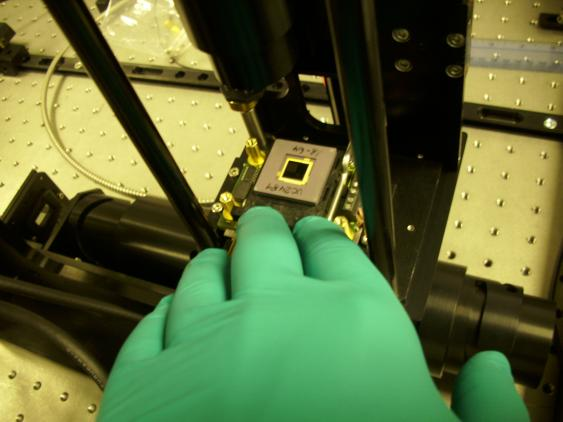
\includegraphics[width=7cm]{mma-plain}
%   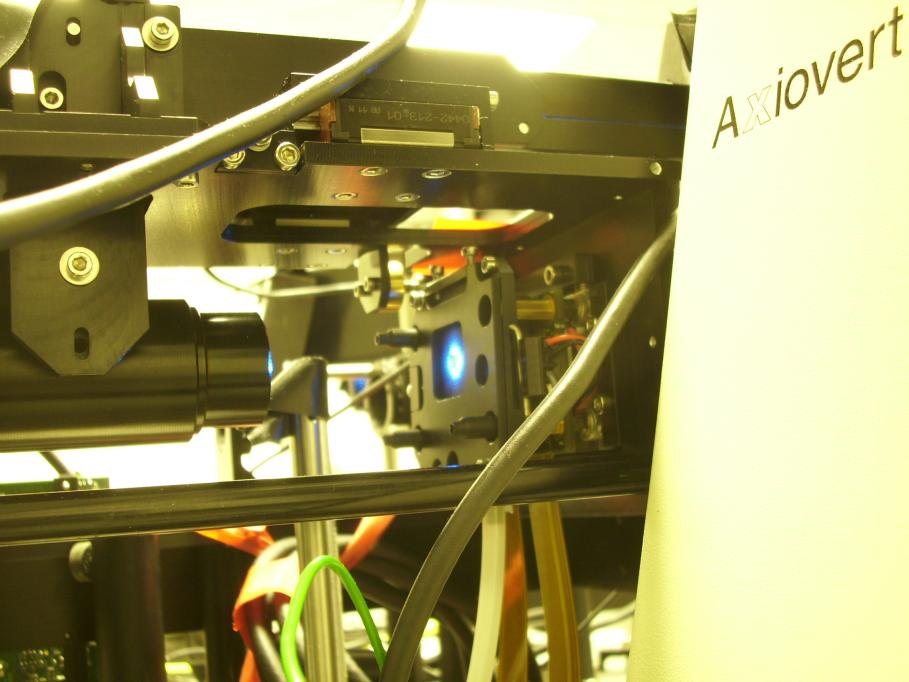
\includegraphics[width=7cm]{mma-ill}
%   \caption{{\bf left:} Micro mirror array chip during installation of
%     the optics. {\bf right:}~Illuminated micro mirror array in the
%     aligned system.}
%   \label{fig:mma-closeup}
% \end{figure}


\section{Mapping between pixels of the focal plane SLM and camera pixels}
\label{sec:map}
A basic prerequisite for measurement with our system is that the
mapping between SLM and camera pixels is known. Only then, the sample
can be irradiated as planned. To measure the mapping, I use a
fluorescent plane sample, turn on individual pixels at position $\r^d$
of the focal plane SLM and acquire camera images, which have bright
spots centered on a camera coordinate $\r^c$.

The fluorescent plane is attached directly to the underside of the
cover slip, ensuring good image quality and no (or negligibly small)
distortion.
\subsection{The rigid transform}
In our experiments, the following transformation with four degrees of
freedom (scaling $s$, rotation angle $\phi$, translation vector $\vect
t=(t_x,t_y)^T$) has proved particularly advantageous:
\begin{align}
  \label{eq:rigid}
  \r^d&=s \textrm{R}_\phi \r^c + \vect t\\
  \textrm{R}_\phi&=\begin{pmatrix}
  \cos\phi & q\sin\phi \\
  -\sin\phi & q\cos\phi \\ 
  \end{pmatrix}
\end{align}
where $\r^d=(r^d_x,r^d_y)^T$ is a point on the display,
$\r^c=(r^c_x,r^c_y)^T$ is a point on the camera and $R_\phi$ is a
rotation matrix. The value of $q$ depends on the arrangement of
mirrors in the beam path. The parameter $q$ is $-1$, if there is a
single axis reflection and it is $+1$ if there is no reflection.
\begin{figure}[!hbt]
  \centering
  \svginput{1}{calib-align}
  \caption{Given $n\ge 4$ camera images of a display showing one
    point.  It is possible to calculate the parameters of the rigid
    transform parameters scaling $s$, rotation angle $\phi$,
    translation vector $\vect t$.}
  \label{fig:calib-align}
\end{figure}

Alternatively, in the beginning we experimented with an affine
transformation. This transform is over-determined, as it includes two
additional degrees of freedom for shear and anisotropic scaling, which
are negligible in our system. Therefore it is difficult to assess the
quality of the calculated affine transform parameters.

With the rigid transform in equation \ref{eq:rigid}, our system can,
however, be modeled very well: The camera is connected to a flange on
the microscope body and can be easily rotated. So when the camera is
moved, ideally, only the rotation angle $\phi$ needs to be
recalibrated. Similarly, the focal length setting of the illumination
tubelens $\textrm{TL}_\textrm{ill}$ mainly affects the scale $s$.
\subsubsection{Computational parameter estimation}
Having measured a set of $n\ge 4$ tuples $(\r^c_i,\r^d_i)$ of camera
and SLM coordinates, the four rigid transform parameters can be
obtained by minimizing the error $\mathcal{Q}$:
\begin{align}
 \mathcal{Q}= \sum_i^n \abs{s \textrm{R}_\phi \r^c_i+\vect t -\r^d_i}^2 \label{eq:rigid-sum}
\end{align}
There are good algorithms to solve this type of least squares problem.
In appendix \ref{sec:map_maxima} I show the source code for the
computer algebra system Maxima % FIXME stephan doesn't like the style
                               % of the reference
\citep{Maxima.sourceforge.net2013}. With ``Maxima'' the implementation
is particularly concise because it transparently calculates all the
necessary derivatives symbolically.

% In addition Maxima can easily be
% integrated in my real-time system.
% not really true for windows
\subsection{Experimental example and image processing}
Now I will show example images to describe the data collection for
measuring the transformation between camera pixels and focal plane
SLM.

For \cma{sample preparation} good results it is useful to have a
fluorescent plane sample that is homogeneous and without empty
(non-fluorescent) holes. I succeeded in making particularly thin and
uniform fluorescent planes with fluorescent beads. I prepared the
sample by drying an undiluted suspension of sub-diffraction,
fluorescent latex beads on a cover slip. This results in expanded areas
with uniform mono-, double- or multi-layers (see
\figref{fig:rigid-pics}).

It \cma{maximize field} is also advantageous if as large an area of
the focal plane SLM as possible is taken into account for the
estimation of the transform's parameters. Therefore I opened the two
diaphragms B0 and B1 (see \figref{fig:memi-real}) completely for the
calibration measurements.  I also kept the mirrors of the pupil plane
SLM undeflected to ensure maximum irradiance in the sample.

For \cma{scanning SLM pixel grid} the calibration I usually do not
only enable individual SLM pixels as this would give very dim images
with \unit[20]{ms} integration time. Instead, I enable pixels in a
circular area around the centre. This results in images as depicted in
\figref{fig:rigid-pics}~right. I acquire 100 such camera images while
moving the circular mask on the focal plane SLM over a $10\times 10$
grid (a disk of 24 focal plane SLM pixels diameter at the positions
$\r^d_{i+j}=(400+50i,500+50j)\ \forall i,j\in [0,99]$). Accidentally a
number of these points fell outside of the illuminated area and were
excluded from further processing.

In Appendix \ref{sec:matlab-spots} I show Matlab code (using the
DIPimage toolbox, \cite{dipimage}) to determine the position of the
bright spot in each camera image. Since the size of the illuminated
areas in the sample is bigger than the diffraction limit and
inhomogeneities of the fluorescent layer therefore will be visible in
the image, the image data must be corrected by dividing the pixel
values by the data of a uniformly illuminated image of the identical
region. Otherwise sample non-uniformities would bias the results of
the localization algorithm.


\comment{
\jpginput{}{o102}{}
\jpginput{}{o035}{}
}

\begin{figure}[!hbt]
  \centering
  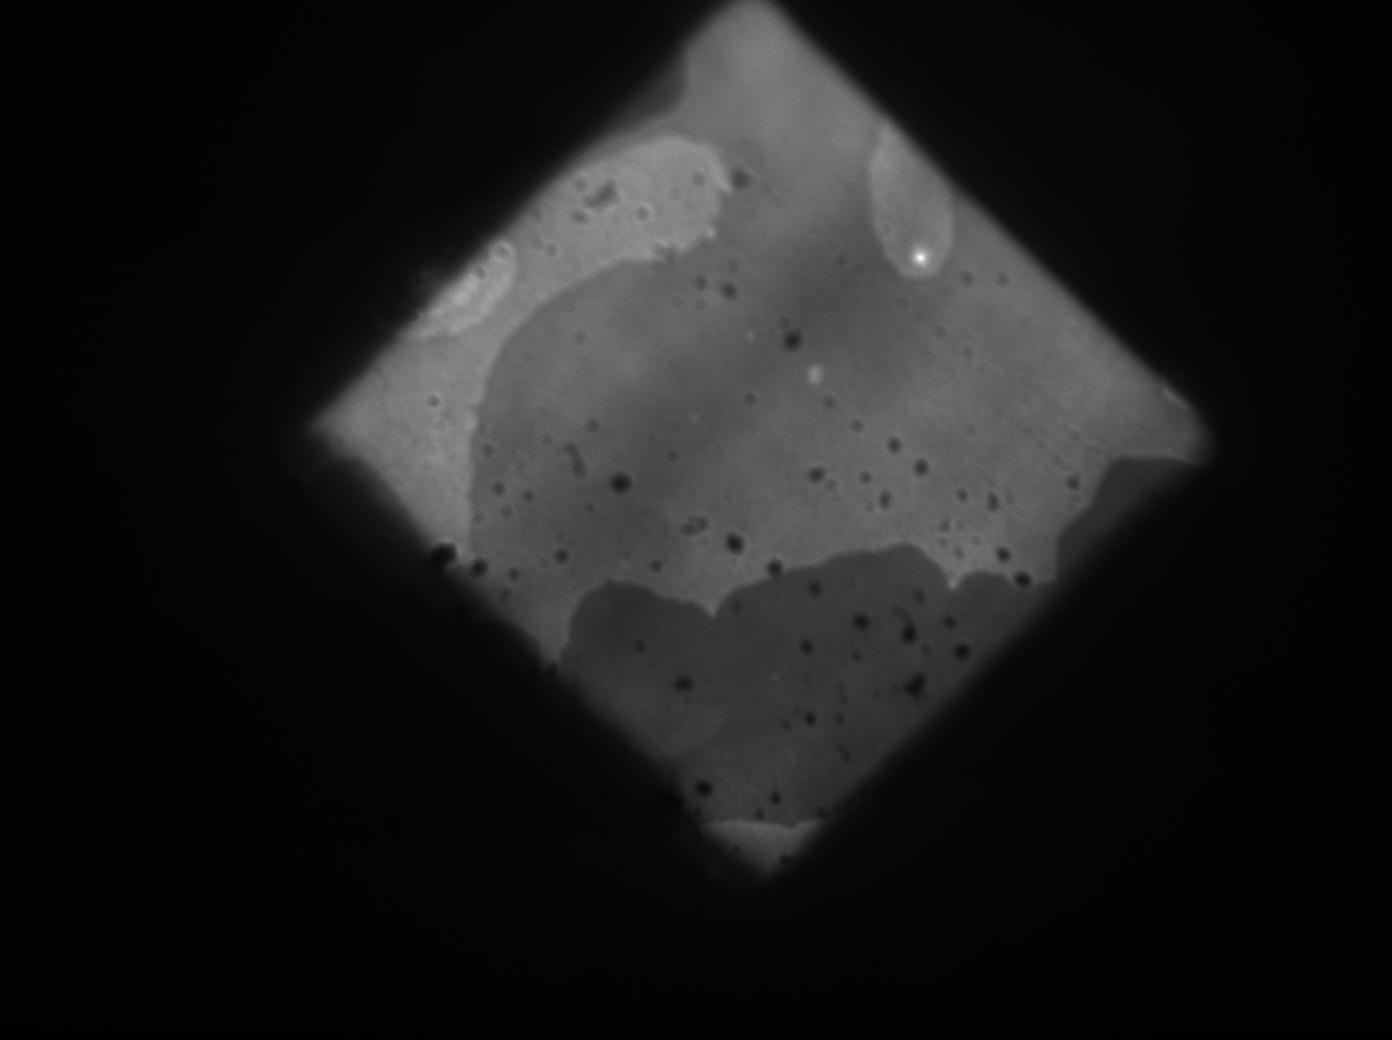
\includegraphics[width=4cm]{o102}\quad
  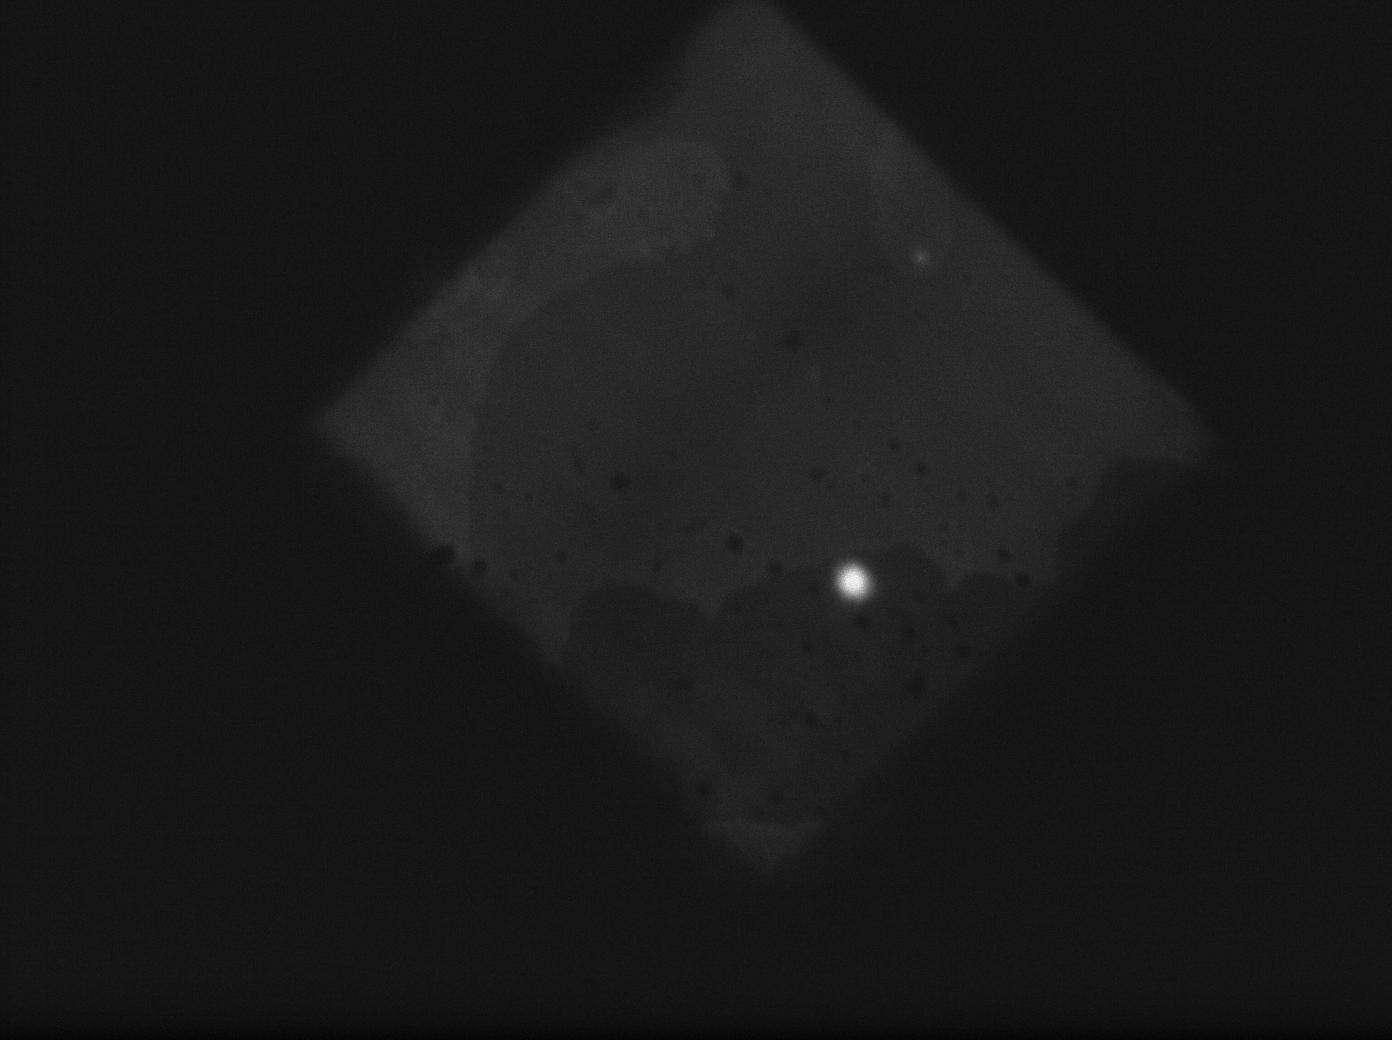
\includegraphics[width=4cm]{o035}
  \caption{{\bf left:} Uniformly illuminated fluorescent plane (mono
    and double layer of yellow beads with \unit[110]{nm} diameter,
    excited with \unit[473]{nm} laser in a 63x/1.47 objective). {\bf
      right:} Image with the the focal plane SLM displaying a disk
    with 24 pixels diameter (corresponding to $\unit[2.4]{\mu m}$ in
    the sample) centred at focal plane SLM position $\r^d = (550,750)$.}
  \label{fig:rigid-pics}
\end{figure}

% i believe the TL_ill is set to r_MMA=3.84mm in BFP 
% f_TLill = 352 mm
% mag_real = mag / f_zeiss * f_TLill 
% pixel-pitch-lcos / mag_real
% one pixel is: 13.62 / 63 * 164.5 / 352 = 101nm


\begin{figure}[!hbt]
  \centering
  \pdfinput{10cm}{rigid-compare}
  \caption{Red ``$+$'' signs indicate where the spots that were
    localized in the camera images end up after a rigid
    transform. There is sufficient agreement with the original
    display positions.}
  \label{fig:rigid-compare}
\end{figure}

\figref{fig:rigid-compare} shows how well the transformed camera
coordinates ($\r^c$, indicated by '$+$' signs) superimpose with the
coordinates of the focal plane SLM pixel grid.


\figref{fig:screen_lcos-calib}~left depicts a pattern of discs that
was displayed on the focal plane SLM and the right figure shows a
superposition of the camera image and the outline of the circles.

\jpginput{7cm}{screen_lcos-calib}{Example of a rigid transform between
  focal plane SLM and camera. {\bf left:} Mask that is displayed on
  the SLM. {\bf right:} Camera image of fluorescent plane illuminated
  by mask. The orange lines indicate the borders of the original
  pattern.}


\subsection{Conclusion}
I have shown the simplest possible transformation to map between the
pixel grid of the camera and the focal plane SLM.

For this I have implemented a calibration routine using a computer
algebra system which would allow for more complicated transformations,
e.g.\ considering image distortion. However, my experiments have shown
that the simple transform is sufficient for our requirements and the
field of view, that the current illumination system supports.

The results of a calibration with this particular transformation can
be easily inverted. Furthermore, the interpretation of the parameters
and their fitting errors is obvious and simple.  In particular, the
fitted transform parameters scaling $s$, rotation $\phi$ and
translation $\vect t$ can be used directly in OpenGL to transform
vector primitives in and elegant way and with negligible computational
effort. I give example code in Appendix \ref{sec:map_opengl}.




%%% Local Variables: 
%%% mode: latex
%%% TeX-master: "kielhorn_memi"
%%% End: 
